\documentclass[11pt]{article}
\usepackage[utf8]{inputenc}
\usepackage[T1]{fontenc}
\usepackage[french]{babel}
\usepackage{amsmath}
\usepackage[bookmarks={true},bookmarksopen={true}]{hyperref}
\usepackage{graphicx}
\usepackage[a4paper]{geometry}
\usepackage{listings}
\usepackage{amssymb}
\usepackage{amsmath,amsfonts}
	\lstset{frame=tb,
		language=Java,
 		aboveskip=3mm,
  		belowskip=3mm,
  		showstringspaces=false,
  		columns=flexible,
  		basicstyle={\small\ttfamily},
  		numbers=none,
 		numberstyle=\tiny\color{gray},
  		keywordstyle=\color{blue},
  		commentstyle=\color{dkgreen},
  		stringstyle=\color{mauve},
  		breaklines=true,
  		breakatwhitespace=true
  		tabsize=3
	}
\pagestyle{plain}
\setlength{\parindent}{5mm}
\usepackage{amsmath}
\usepackage{color}
\definecolor{dkgreen}{rgb}{0,0.6,0}
\definecolor{gray}{rgb}{0.5,0.5,0.5}
\definecolor{mauve}{rgb}{0.58,0,0.82}



\title{\textbf{Projet LSINF1121 -  Algorithmique et structures de données\\ - \\ Rapport intermédiaire Mission 6} \\ {\large Groupe 26}}
\author{Laurian \bsc{Detiffe} \\(6380-12-00)\and Sundeep \bsc{Dhillon} \\(6401-11-00)\and Alexis \bsc{Macq} \\ (5910-12-00) \and Xavier \bsc{Pérignon} \\ (8025-11-00)\and Thibaut \bsc{Piquard}\\(4634-13-00)\and Thomas \bsc{Wyckmans} \\ (3601-12-00)}
\date{date}
\date{\vspace*{25mm}

\includegraphics[scale=0.75]{logo.jpg}\\
		\vspace*{30mm}
		\begin{center}
		Année académique 2015-2016 \\	
		\end{center}}

\begin{document}
\thispagestyle{empty}

\maketitle
\thispagestyle{empty}
%\tableofcontents
%\setcounter{tocdepth}{3}
%\setcounter{page}{1}
%\newpage

\section*{Questions et réponses}
\begin{enumerate}

\item

\item  

\item 

\item 

\item 

\item 

\item 

\item 

\item 

\item 

\item Soit $G$ un graphe avec des poids potentiellement négatif mais il n’y a pas de
cycle négatif. Je cherche le chemin le plus court entre un noeud $u$ et un noeuds $v$.
J’ai à ma disposition une implémentation de Dijkstra qui ne permet pas de gérer
les poids négatifs. Il me suffit dès lors d’augmenter tous les poids d’une même
quantité correspondant a la valeur absolue du plus petit poids et d’appliquer
Dijkstra sur ce graphe. Cette méthode est-elle valable ? Si non, montrez un contre
exemple. (Xavier)\\

Non, c'est méthode n'est pas valable. Par exemple, considérons le graphe où il existe deux chemins de A vers B, l'un traversant un seul arc de longueur 2, et l'autre traversant des arcs de longueur 1, 1 et -2. Le deuxième chemin est plus court, mais si on augmente de 2 tous les poids des arcs (valeur absolue du plus petit poids), le premier chemin a maintenant une longueur de 4, et le second a une longueur de 6, inversant le chemin le plus courts.
\begin{center}
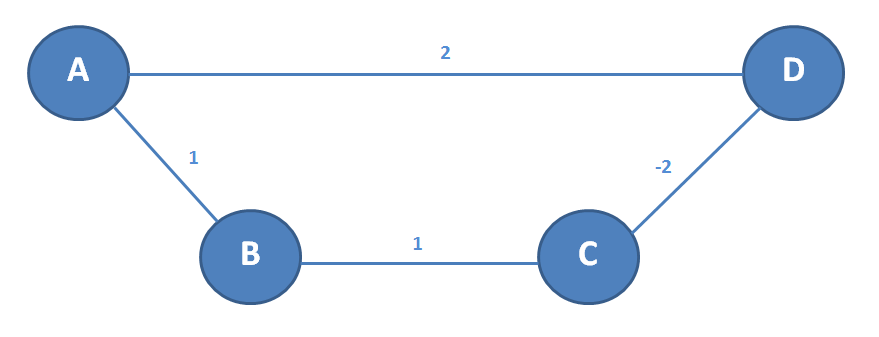
\includegraphics[scale=0.5]{dijk.PNG} 
\end{center}
Cette méthode ne fonctionnera que si tous les chemins possibles entre les deux noeuds utilisent le même nombre d'arcs.\\

\item Soit $G$ un graphe avec des poids positifs. Je cherche le chemin le plus long entre
un noeud $u$ et un noeuds $v$. J’ai à ma disposition l’implémentation de Bellman-
Ford (qui supporte les poids négatifs). Il me suffit dès lors de calculer le plus
court chemin sur le même graphe avec l’opposé des poids. Est-ce que cette méthode
est valable ? Si non pouvez-vous proposer une méthode pour le calcul de
plus long chemin ? Votre méthode s’applique-t-elle à tous les graphes ? Si non
quels-types particuliers de graphes peut-elle gérer ? (Xavier)\\

Cette méthode est valable pour certains graphes. Le principe le plus important pour l'utilisation de cette méthode est qu'il n'y ait pas de cycle dans le graphe, dans laquelle les arcs ont une somme négative. Dans ce cas, une boucle infinie serait générée et aucun plus long chemin ne serait trouvé.

\end{enumerate}
\end{document}